\documentclass[14pt,fleqn]{extarticle}
\usepackage[T2A,T1]{fontenc}
\usepackage[utf8]{inputenc}
\usepackage[russian]{babel}
\usepackage{amsmath}
\usepackage{graphicx}
\usepackage{tabularx}
\usepackage{boldline}
\usepackage{makecell}
\usepackage{arydshln}
\usepackage{mathtools}
\usepackage{centernot}
\usepackage{enumitem}
\usepackage{nccmath}
\usepackage{amssymb}
\usepackage[a4paper, total={6.5in, 9.5in}]{geometry}

\graphicspath{ {./images/} }
\setlength{\mathindent}{0pt}
\setlength\parindent{0pt}

\def\at{
	\left.
	\vphantom{\int}
	\right|
}


\begin{document}
	\begin{titlepage}
		
\includegraphics[scale=0.12]{logo}
		\begin{center}
			\textbf{МИНОБРНАУКИ РОССИИ}\\
			\vspace{0.2cm}
			\textbf{Федеральное государственное бюджетное образовательное учреждение высшего образования}\\
			\textbf{<<САНКТ-ПЕТЕРБУРГСКИЙ ГОСУДАРСТВЕННЫЙ ЭКОНОМИЧЕСКИЙ УНИВЕРСИТЕТ>>}\\
			\vspace{0.6cm}
			Факультет информатики и прикладной математики\\
			Кафедра прикладной математики и экономико-математических методов\\
			\vspace{1cm}
			\textbf{ОТЧЁТ}\\
			по дисциплине:\\
			\textbf{<<Модели экономической динамики>>}\\
			на тему:\\
			\textbf{<<Кластеризация экономик. Динамика экономики Японии.>>}\\
		\end{center}
		\vspace{1cm}
		Направление: 01.03.02\\
		Обучающийся: Бронников Егор Игоревич\\
		Группа: ПМ-1901\\
		\vfill
		\begin{center}
			Санкт-Петербург\\
			2022\\
		\end{center}
	\end{titlepage}
    \subsubsection*{Задание}
    
    Выполнить кластеризацию экономик, используя следующий набор показателей (отдельно за 2019, 2013 и с использованием среднего темпового показателя на временном интервале с 2013 по 2019):
    \begin{itemize}[topsep=0pt,itemsep=-1ex,partopsep=1ex,parsep=1ex]
		\item темпы роста ВВП;
		\item подушевой ВВП, темп роста ВВП;
		\item подушевой ВВП, темпы роста ВВП, темп инфляции.
	\end{itemize}

	Проанализировать полученное распределение по кластерам, миграцию между кластерами, дать содержательную интерпретацию результатов кластеризации.
	
	\subsubsection*{Решение}
	
	Данные были взяты с сайта Всемирного банка.\\
	Первый этап заключался в выделении объединений стран и исключении их из исходного набора данных. Был создан файл с наименованиями этих объединений. (Рисунок \ref{fig:cluster_county_alliances})
	\begin{figure}[h]
		\centering 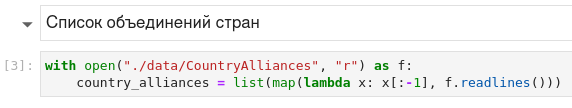
\includegraphics[scale=0.6]{cluster_county_alliances}
		\caption{Заполнения списка объединений стран}
		\label{fig:cluster_county_alliances}
	\end{figure}

	Далее были загружены датасеты с темпами роста ВВП (\%), подушевого ВВП (текущий US\$), темпами инфляции (\%). (Рисунок \ref{fig:cluster_dataset_example})
	\begin{figure}[h]
		\centering 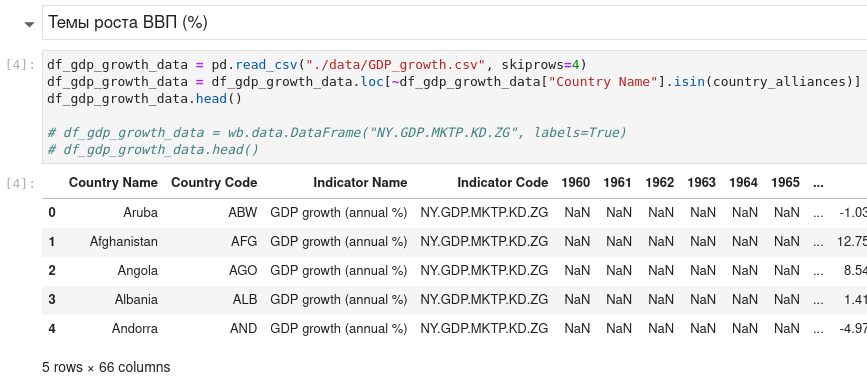
\includegraphics[scale=0.45]{cluster_dataset_example}
		\caption{Пример подгруженных данных}
		\label{fig:cluster_dataset_example}
	\end{figure}
	
	\newpage
	
	На следующем этапе было решено начать с \textit{кластеризации стран на основании темпов роста ВВП за 2019 год}.\\
	
	Были отобраны соответствующие данные. Также были удалены страны, которые не содержат данных. (Рисунок \ref{fig:cluster_select_correct_data})
	
	\begin{figure}[h]
		\centering 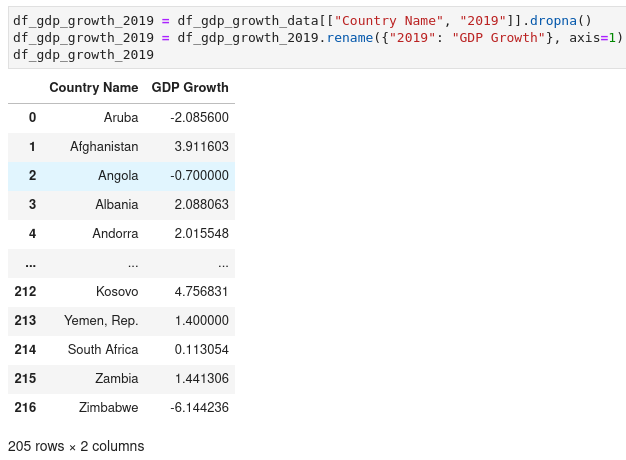
\includegraphics[scale=0.5]{cluster_select_correct_data}
		\caption{Пример отбора необходимых данных}
		\label{fig:cluster_select_correct_data}
	\end{figure}

	Далее была построена дендрограмма и на основании получившегося результата было решено взять для рассмотрения 5 кластеров, для более качественной интерпретации. (Рисунок \ref{fig:cluster_dendrogram})
	
	\begin{figure}[h]
		\centering 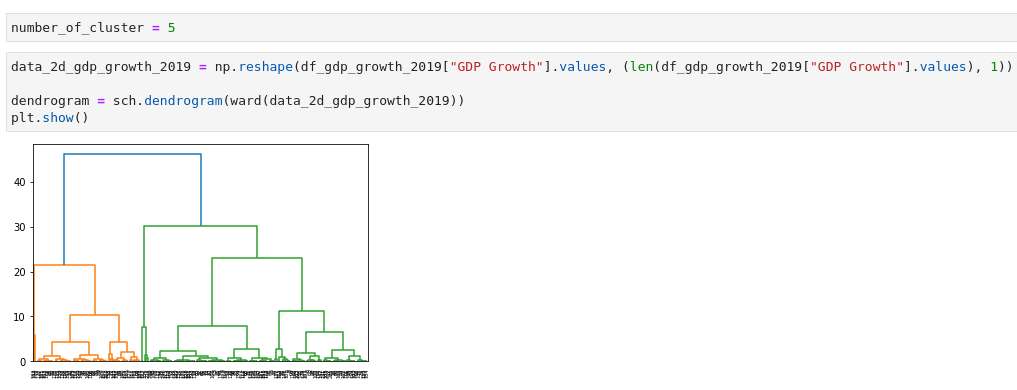
\includegraphics[scale=0.5]{cluster_dendrogram}
		\caption{Построение дерева дендрограммы}
		\label{fig:cluster_dendrogram}
	\end{figure}

	\newpage
	
	Далее происходил процесс кластеризации методом \textit{AgglomerativeClustering}. (Рисунок \ref{fig:cluster_clustering})
	
	\begin{figure}[h]
		\centering 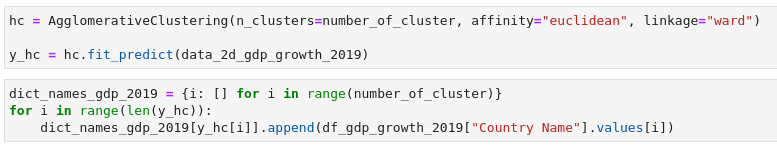
\includegraphics[scale=0.5]{cluster_clustering}
		\caption{Кластеризация данных}
		\label{fig:cluster_clustering}
	\end{figure}

	После чего можно вывести название стран, которые попали в конкретный кластер. (Рисунок \ref{fig:cluster_country_names})
	
	\begin{figure}[h]
		\centering 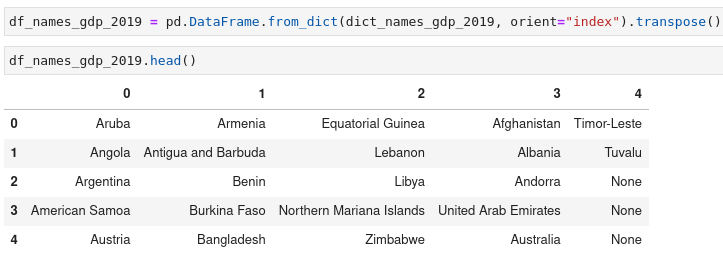
\includegraphics[scale=0.5]{cluster_country_names}
		\caption{Распределение стран по кластерам (названия)}
		\label{fig:cluster_country_names}
	\end{figure}

	Также можно вывести значение темпов роста ВВП стран в кластерах. (Рисунок \ref{fig:cluster_country_values})
	
	\begin{figure}[h]
		\centering 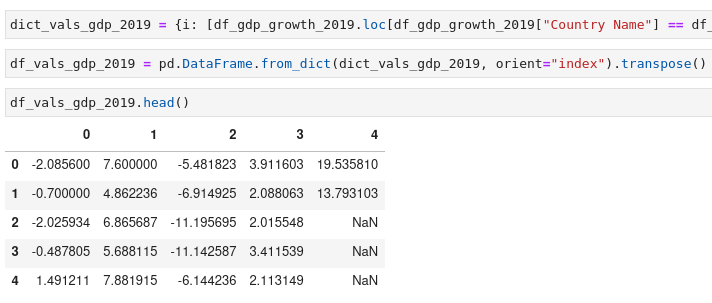
\includegraphics[scale=0.5]{cluster_country_values}
		\caption{Распределение стран по кластерам (значения)}
		\label{fig:cluster_country_values}
	\end{figure}
	
	\newpage
	
	Можно выделить численные характеристики каждого получившегося кластера: количество стран в кластере, минимальное значение, максимальное значение и среднее значение. (Рисунок \ref{fig:cluster_cluster_features})

	\begin{figure}[h]
		\centering 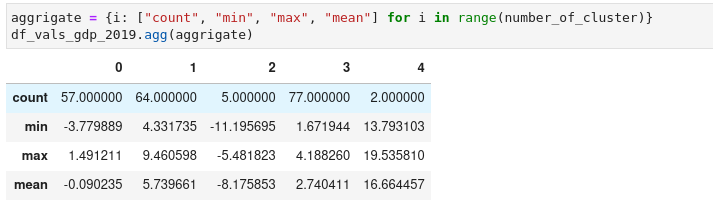
\includegraphics[scale=0.6]{cluster_cluster_features}
		\caption{Численные характеристики кластеров}
		\label{fig:cluster_cluster_features}
	\end{figure}

	В данном случае можно выделить, что в 4 кластер попали страны, которые имеют очень высокие темпы роста ВВП, в 1 кластер попали страны с высоким темпом роста ВВП, в 3 кластер попали страны со средними темпами роста ВВП, в 0 кластер попали страны с низким темпом роста ВВП, а во 2 кластер попали страны с очень низким темпом роста ВВП.\\
	
	Также получившиеся данные сохраняются в \textit{Excel}-файл. На 1 листе будут отображены наименования стран распределённые по кластерам, а на 2 листе будут отражены соответствующие им показатели. (Рисунок \ref{fig:cluster_save_data})
	
	\begin{figure}[h]
		\centering 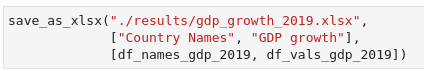
\includegraphics[scale=0.6]{cluster_save_data}
		\caption{Сохранение получившихся результатов в Excel-файле}
		\label{fig:cluster_save_data}
	\end{figure}

	Далее данные шаги повторяются для каждого из годов и соответствующих объединений показателей как указано в условии задачи.\\
	
	Единственное что стоит отметить, что при рассмотрении факторов, которые имеют разные единицы измерения (\% и текущие US\$), перед кластеризацией стоит провести процесс стандартизации. Также стоит отметить, что когда мы рассматриваем средние показатели с 2013 года по 2019 год стоит рассматривать среднее геометрическое показателей если соответствующая величина выражена в \% соотношении.
	
	\newpage
	
	На основании получившихся данных, была рассмотрена миграция стран по кластерам.\\
	
	В качестве примера рассмотрим миграцию стран по темпам роста ВВП среди стран, которые показали средний темпы роста в 2013 году.\\
	
	Страны, оставшиеся в кластере средних темпов роста ВВП. (Рисунок \ref{fig:cluster_mean_mean})
	
	\begin{figure}[h]
		\centering 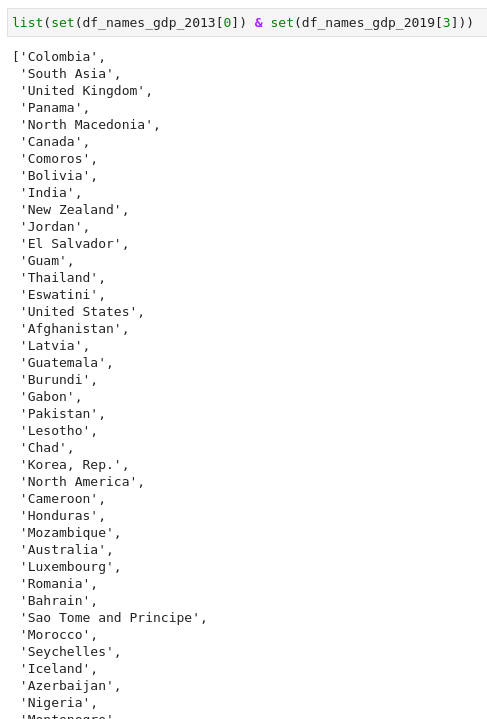
\includegraphics[scale=0.5]{cluster_mean_mean}
		\caption{Оставшиеся в своём кластере}
		\label{fig:cluster_mean_mean}
	\end{figure}

	\newpage

	Страны, мигрировавшие в кластер с высокими темпами роста ВВП. (Рисунок \ref{fig:cluster_mean_high})

	\begin{figure}[h]
		\centering 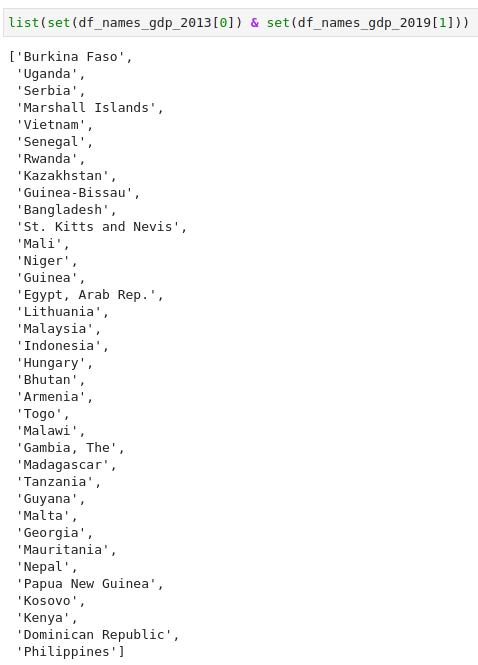
\includegraphics[scale=0.45]{cluster_mean_high}
		\caption{Мигрировавшие в кластер с высокими темпами роста}
		\label{fig:cluster_mean_high}
	\end{figure}

	Страны, мигрировавшие в кластер с очень высокими темпами роста ВВП. (Рисунок \ref{fig:cluster_mean_very_high})

	\begin{figure}[h]
		\centering 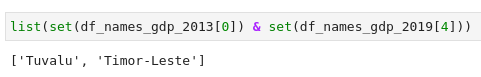
\includegraphics[scale=0.5]{cluster_mean_very_high}
		\caption{Мигрировавшие в кластер с очень высокими темпами роста}
		\label{fig:cluster_mean_very_high}
	\end{figure}

	Страны, мигрировавшие в кластер с очень низкими темпами роста ВВП. (Рисунок \ref{fig:cluster_mean_very_low})

	\begin{figure}[h]
		\centering 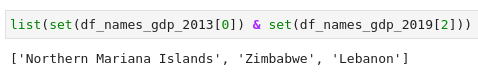
\includegraphics[scale=0.5]{cluster_mean_very_low}
		\caption{Мигрировавшие в кластер с очень низкими темпами роста}
		\label{fig:cluster_mean_very_low}
	\end{figure}

	\newpage
	
	Страны, мигрировавшие в кластер с низкими темпами роста ВВП. (Рисунок \ref{fig:cluster_mean_low})
	
	\begin{figure}[h]
		\centering 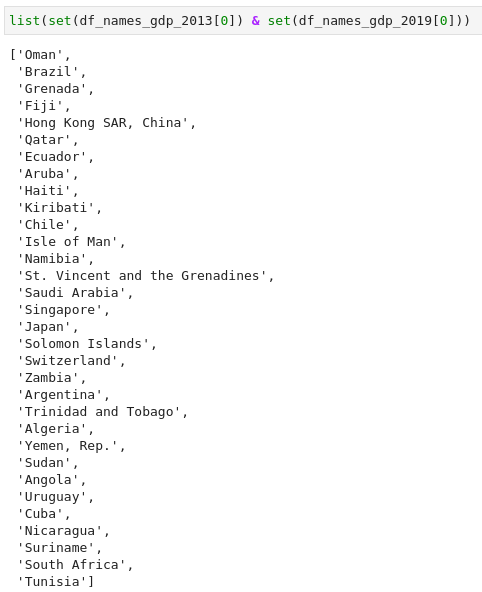
\includegraphics[scale=0.45]{cluster_mean_low}
		\caption{Мигрировавшие в кластер с низкими темпами роста}
		\label{fig:cluster_mean_low}
	\end{figure}

	Аналогичным образом были получены результаты для всех остальных миграций по показателям и по их принадлежности к конкретному кластеру.
	
	\newpage
	
	\subsubsection*{Задание}
	
	Выбрать значимые показатели для рассмотрения динамики экономики страны, сделать прогнозы и описать полученные результаты по миграции данной страны в кластерах.
	
	\subsubsection*{Решение}
	
	В качестве рассматриваемой страны была выбрана Япония.\\
	
	Были рассмотрены следующие показатели:
	\begin{enumerate}[topsep=0pt,itemsep=-1ex,partopsep=1ex,parsep=1ex]
		\item численность людей (тыс.)
		\item численность молодого населения 0-14 (\% от общей численности)
		\item темпы роста ВВП (\%)
		\item уровень безработицы (\% от всей рабочей силы)
		\item уровень экспорта (\% от ВВП)
		\item уровень импорта (\% от ВВП)
		\item подушевой ВВП (текущих US\$)\\
	\end{enumerate}

	Эти данные были взяты с сайта Всемирного банка [9.10.2022]. (Рисунок \ref{fig:japan_data})
	
	\begin{figure}[h]
		\centering 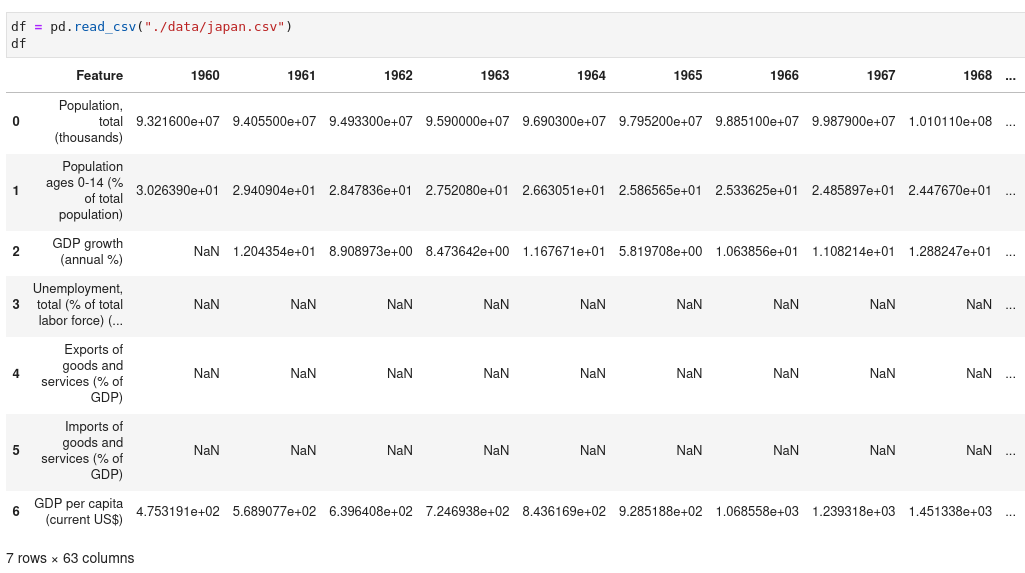
\includegraphics[scale=0.45]{japan_data}
		\caption{Выбранные показатели Японии с 1960 года по 2021 год}
		\label{fig:japan_data}
	\end{figure}

	\newpage
	
	Далее был рассмотрен каждый показатель отдельно.\\
	На основе данных можно построить график как менялась численность населения. (Рисунок \ref{fig:japan_population_plot})
	
	\begin{figure}[h]
		\centering 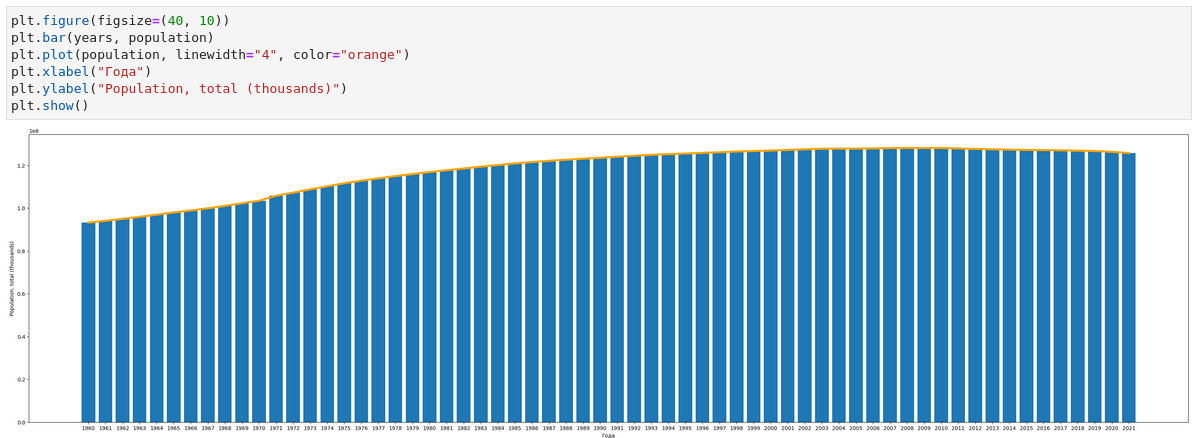
\includegraphics[scale=0.42]{japan_population_plot}
		\caption{Динамика численности населения Японии с 1960 года по 2021 год}
		\label{fig:japan_population_plot}
	\end{figure}

	Можно заметить, что до 2005-2006 года наблюдался рост численности людей, после уровень популяции вышел на плато, а затем (с 2010 года) начал постепенно убывать.\\
	
	Стоит также проанализировать и <<молодую>> часть населения Японии. (Рисунок \ref{fig:japan_young_population_plot})
	
	\begin{figure}[h]
		\centering 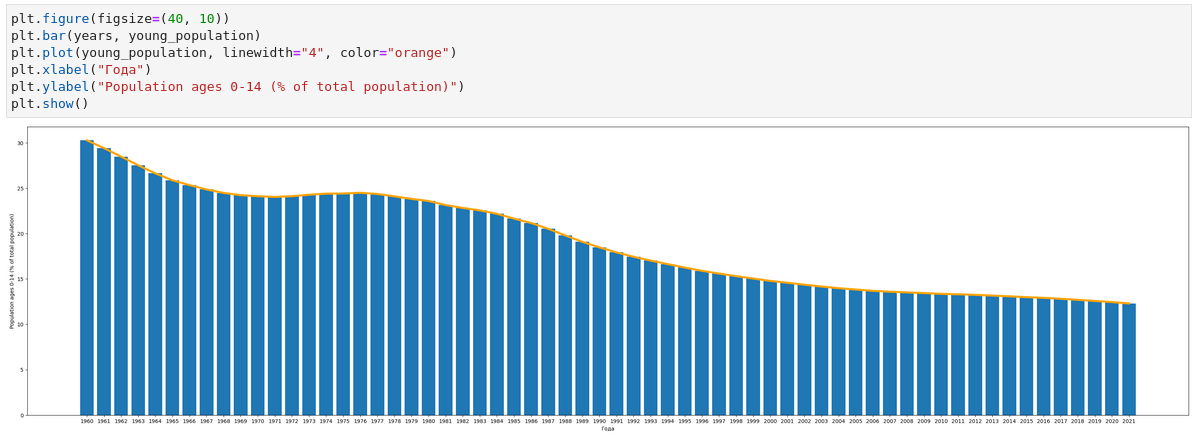
\includegraphics[scale=0.42]{japan_young_population_plot}
		\caption{Динамика молодого населения Японии с 1960 года по 2021 год}
		\label{fig:japan_young_population_plot}
	\end{figure}

	На графике видно, что детей становится с каждым годом всё меньше и меньше.
	
	\newpage
	
	Проблема демографии не обошла и Японию, по демографическим пирамидам можно заметить, что на сегодняшний день основную часть населения составляют люди в <<зрелом>> возрасте. Как можно заметить из возрастно-половых пирамид, если ничего не поменяется, то прогнозируют, что к 2050 году в Японии сократится население на 20 миллионов человек. (Рисунок \ref{fig:japan_pyramid})
	
	\begin{figure}[h]
		\centering 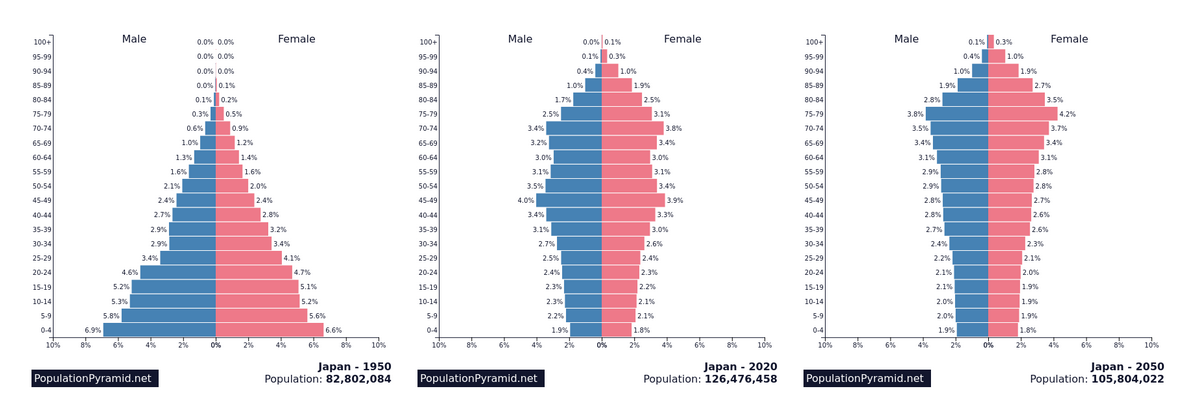
\includegraphics[scale=0.43]{japan_pyramid}
		\caption{Возрастно-половые пирамиды}
		\label{fig:japan_pyramid}
	\end{figure}
	
	Далее было рассмотрено изменение темпов роста ВВП. (Рисунок \ref{fig:japan_gdp_growth_plot})
	
	\begin{figure}[h]
		\centering 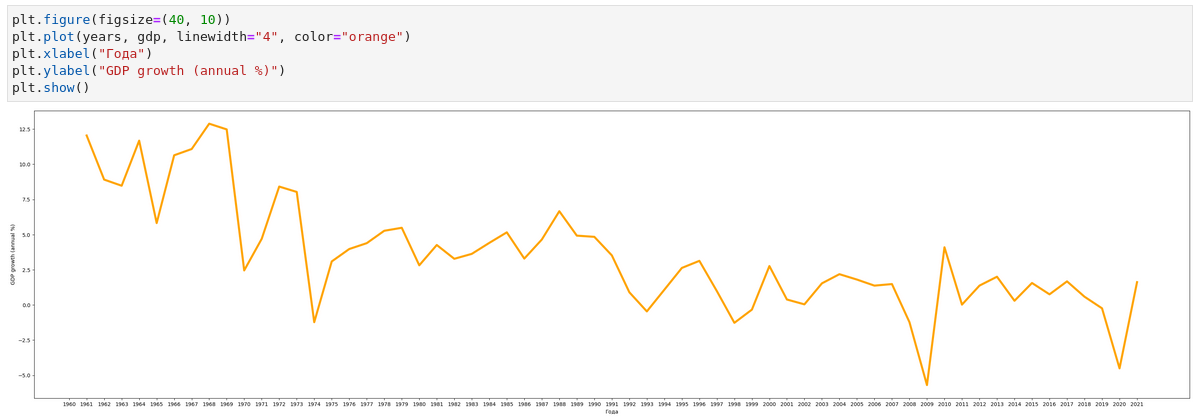
\includegraphics[scale=0.43]{japan_gdp_growth_plot}
		\caption{Динамика темпов роста ВВП Японии с 1960 года по 2021 год}
		\label{fig:japan_gdp_growth_plot}
	\end{figure}
	
	Можно заметить что с середины 1950 до 1973 года темпы прироста ВВП были достаточно велики, составляли более 10\% ежегодно и это были самые высокие показатели прироста ВВП среди развитых стран того времени. Этот феномен называют <<Японское экономическое чудо>>.
	
	\newpage
	
	Причины данного феномена:
	\begin{itemize}[topsep=0pt,itemsep=-1ex,partopsep=1ex,parsep=1ex]
		\item дешевизна рабочей силы
		\item объединение производителей, поставщиков ресурсов, сбытчиков продукции и банков в тесно связанные группы
		\item взаимовыгодные отношения предпринимателей с правительством
		\item Корейская война, поставка вооружения США через Японию
		\item отсутствие военных расходов у Японии (отказ от милитаристского бюджета). В 1972 году его доля составила только 1\% от ВНП
		\item освоение японской наукой новых технологий, скупка патентов и лицензий
		\item \dots\\
	\end{itemize}

	Также можно заметить, что присутствуют спады, а именно в 1973 году случился Нефтяной кризис, а так как Япония в те годы делала упор на химическую промышленность, в том числе и переработку нефти, то на их экономики это тоже сказалось. Ещё имеются спады в 2008 году и 2020 году, в 2008 году произошёл Мировой кризис, а в 2020 году был COVID-19.\\
	
	Если посмотреть, то за исключением кризисов был стабильный ежегодный прирост ВВП в среднем на 2.24\%, что достаточно хорошо.\\
	
	Следующий фактор, который был проанализирован -- это динамика уровня безработицы. (Рисунок \ref{fig:japan_unemployment_plot})
	
	\begin{figure}[h]
		\centering 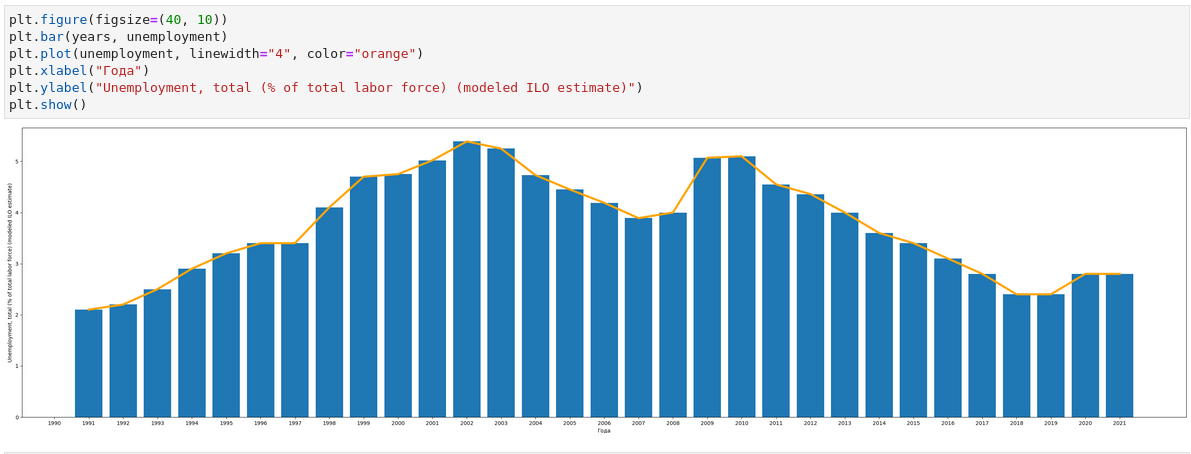
\includegraphics[scale=0.42]{japan_unemployment_plot}
		\caption{Динамика уровня безработицы Японии с 1991 года по 2021 год}
		\label{fig:japan_unemployment_plot}
	\end{figure}

	Можно заметить, что уровень безработицы в Японии достаточно низкий и в среднем составляет 3.7\%.
	
	\newpage
	
	Далее рассматривалась динамика объёмов экспорта. (Рисунок \ref{fig:japan_export_plot})
	
	\begin{figure}[h]
		\centering 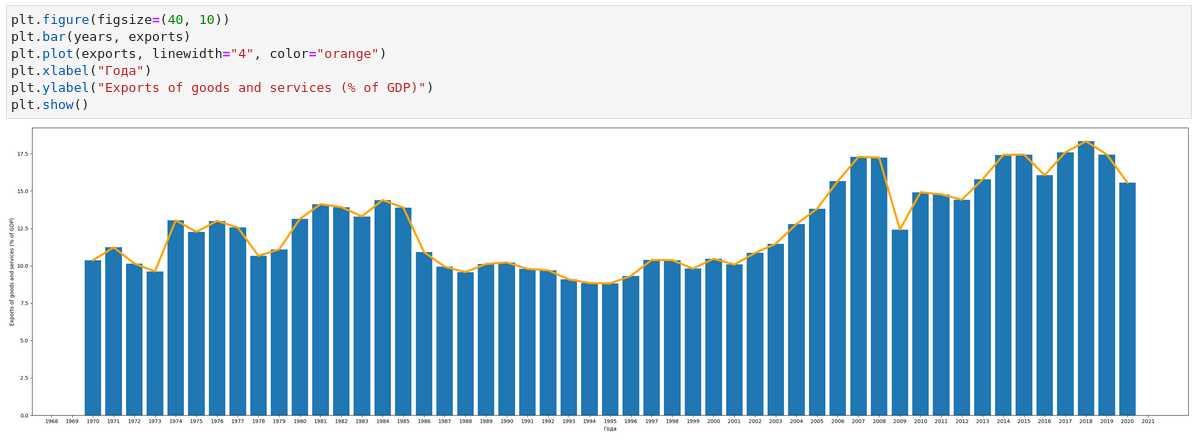
\includegraphics[scale=0.42]{japan_export_plot}
		\caption{Динамика объёмов экспорта Японии с 1970 года по 2020 год}
		\label{fig:japan_export_plot}
	\end{figure}

	Страна не очень богата природными ресурсами, но тем не менее она является одним из главных мировых экспортёров в отраслях:
	\begin{itemize}[topsep=0pt,itemsep=-1ex,partopsep=1ex,parsep=1ex]
		\item робототехники
		\item автомобилестроения
		\item электронно-вычислительной техники
		\item бытовой химии\\
	\end{itemize}

	И также были рассмотрены изменения уровня объёма импорта. (Рисунок \ref{fig:japan_import_plot})
	
	\begin{figure}[h]
		\centering 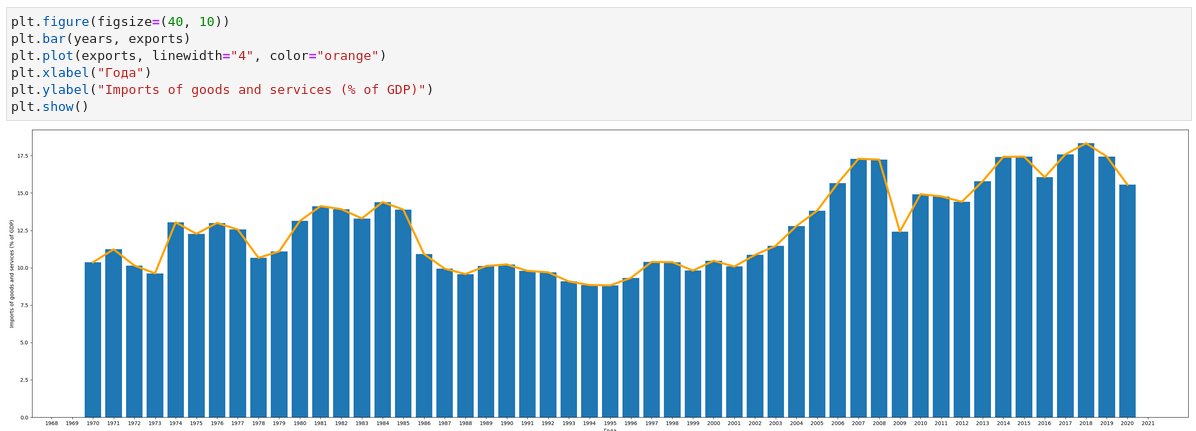
\includegraphics[scale=0.42]{japan_import_plot}
		\caption{Динамика объёмов импорта Японии с 1970 года по 2020 год}
		\label{fig:japan_import_plot}
	\end{figure}

	\newpage
	
	Основными товарами импорта являются:
	\begin{itemize}[topsep=0pt,itemsep=-1ex,partopsep=1ex,parsep=1ex]
		\item минеральные ресурсы
		\item текстильные товары
		\item металло-продукция
		\item продукты питания\\
	\end{itemize}

	Последний рассмотренный фактор -- это динамика подушевого ВВП. (Рисунок \ref{fig:japan_gdp_per_capita_plot})
	
	\begin{figure}[h]
		\centering 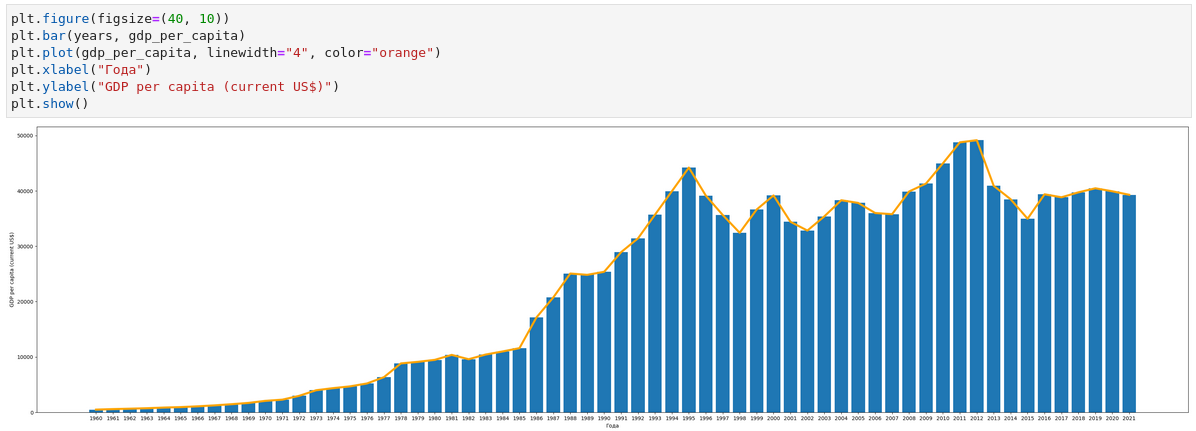
\includegraphics[scale=0.42]{japan_gdp_per_capita_plot}
		\caption{Динамика объёмов подушевого ВВП Японии с 1970 года по 2020 год}
		\label{fig:japan_gdp_per_capita_plot}
	\end{figure}

	Можно видеть, что когда Япония проиграла Вторую мировую войну, то страна была разрушена и ВВП был достаточно низок, а численность населения была большой. Однако потом страна начала наращивать темпы роста ВВП и произошло <<Японское экономическое чудо>>, после чего темпы подушевого ВВП выросли и сейчас достаточно стабильны.\\
	
	Далее были построены прогнозы на 10 лет для каждого из признаков с помощью модели прогнозирования \textit{SARIMAX}. Для каждого признака были подобраны оптимальные значения $p$ и $q$ c помощью графиков автокорреляции и частичной автокорреляции.\\
	
	\newpage
	
	Первым было спрогнозировано изменение уровня безработицы. (Рисунок \ref{fig:japan_unemployment_plot_forecast})
	
	\begin{figure}[h]
		\centering 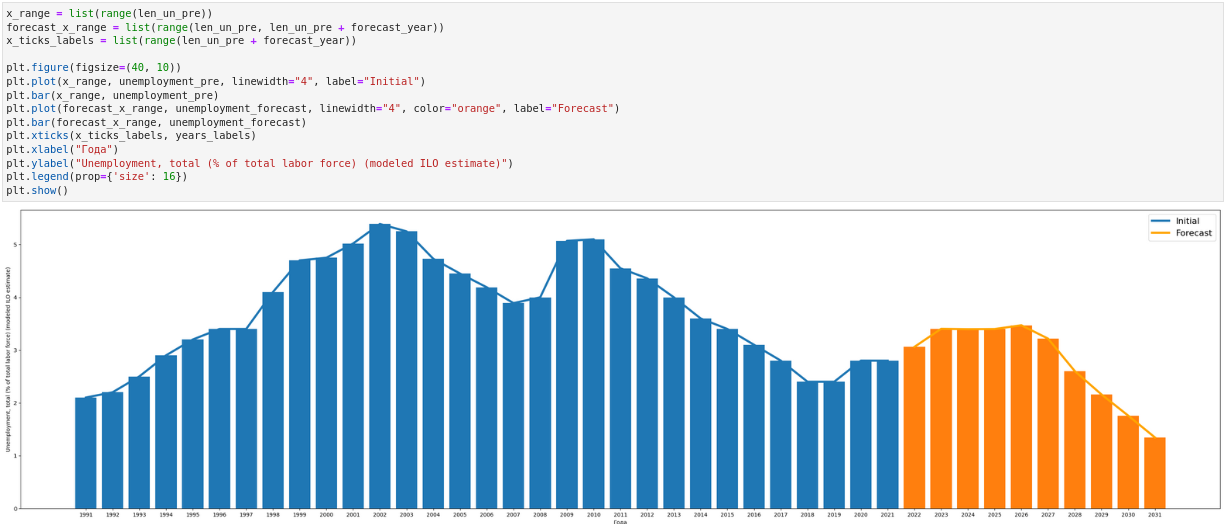
\includegraphics[scale=0.42]{japan_unemployment_plot_forecast}
		\caption{Прогноз динамики уровня безработицы Японии на 10 лет}
		\label{fig:japan_unemployment_plot_forecast}
	\end{figure}

	Можно видеть, что в ближайшие 10 лет будет ожидаться сначала стабильный уровень безработицы, а затем он будет уменьшаться.
\end{document}
